\lstdefinelanguage{llang}{
keywords={for, while, if, then, else, struct, typedef, register, const, include, define, case, break, return, default, switch},
sensitive=true,
%%basicstyle=\small,
commentstyle=\scriptsize\rmfamily,
keywordstyle=\ttfamily\underbar,
identifierstyle=\ttfamily,
basewidth={0.5em,0.5em},
columns=fixed,
fontadjust=true,
literate={->}{{$\to$}}1
}

\lstset{
language=llang
}

\title{Построение корневого множества указателей для сборки мусора}
%
\titlerunning{Построение корневого множества}
\author{Березун Даниил Андреевич}
%
\authorrunning{Д.А.Березун} % abbreviated author list (for running head)
%
%%%% list of authors for the TOC (use if author list has to be modified)
\tocauthor{Д.А.Березун}
%
\institute{Санк-Петербургский государственный университет\\
\email{danya.berezun@gmail.com}}

\maketitle              % typeset the title of the contribution

\begin{abstract}
В работе рассматриваются основные проблемы, возникающие при попытке построения
точного корневого множества указателей для языка С, и описывается способ
его построения при использовании компилятора GCC.
\end{abstract}
%

\section*{Введение}

\emph{Сборка мусора} является одним из способов автоматического управления памятью, при котором освобождение памяти 
выводится из-под контроля ПО на прикладном уровне. При автоматическом управлении программист не может явно влиять на 
распределение объектов в памяти, у него есть лишь косвенные способы сделать это с помощью использования тех или иных
языковых конструкций. В идеальном случае, для рационального использования памяти необходимо освобождать память, занимаемую 
объектами, которые более не будут использованы программой. Поскольку точно определить, что объект не будет использован в дальнейшем, 
невозможно, на практике используют критерий доступности. \emph{Доступность} --- это консервативное приближение используемости. 
\emph{Мусором}, в таком случае, называют объект, все пути доступа к которому уже разрушены, а память из-под него ещё не освобождена. 
В некоторое, заранее определенное время, например, в простейшем случае, когда перестаёт хватать свободной памяти, выполнение 
программы временно приостанавливается и запускается процесс \emph{сборки мусора}, который освобождает всю или ту, что возможно, 
память, занятую мусором, после чего управление возвращается обратно программе. \emph{Сборщиком мусора} называется компонент, 
производящий \emph{сборку мусора}.

Есть несколько требований, которые должны быть выполнены для реализации сборки мусора:

\begin{enumerate}
\item Должна присутствовать возможность определить все указатели из любого объекта на другие элементы кучи.
\item Отсутствуют операции(арифметические, логические и т.п.) над указателями.
\end{enumerate}

В таких языках, как LISP или JAVA все условия соблюдаются, и в них успешно используется технология сборки мусора,
в то время как, например, в языке C не все условия выполняются. В языках, где не соблюдаются некоторые условия, возможна исключительно
\emph{консервативная сборка мусора}. \emph{Консервативной} называется такая сборка мусора, при которой любой элемент данных, значение 
которого может быть истолковано как указатель на некоторый элемент кучи, считается  \emph{допустимым указателем}, т.е. указателем, который 
указывает на некоторый объект кучи и был получен как результат функции выделения памяти. Консервативный подход к сборке мусора не позволяет 
собрать весь мусор, что может стать проблемой при обработке большого количества данных.

Процесс \emph{сборки мусора}, в простейшем случае, делят на три этапа:
\begin{enumerate}
\item \emph{Построение корневого множества}. На этом этапе строится множество объектов, которые считаются изначально доступными. 
Данное построение аксиоматично, т.е. основывается на некотором наборе правил, согласно которым те или иные элементы считаются доступными.
\item \emph{Маркировка}. Начиная с множества, построенного на предыдущем этапе, происходит сканирование памяти, и все объекты, до которых 
возможно добраться из построенного корневого множества, считаются доступными; оставшиеся объекты считаются мусором.
\item \emph{Освобождение}. Происходит сканирование кучи, в течение которого память из-под всех элементов, помеченных как мусор или не отмеченных 
как доступные, освобождается.
\end{enumerate}

Существуют разнообразные схемы сборки мусора, но в них всех есть построение корневого множества.

Во всех источниках, описывающих процесс сборки мусора, этап построения корневого множества описывается на уровне лишь упоминания о нём или же 
попросту упускается. Данное обстоятельство связано с тем, что построение корневого множества является платформозависимой операцией; 
тем не менее принципы его построения остаются неизменными.

Все сказанное в данной работе верно для языков, использующих программный стек для хранения записей активации фукций (C, C++, C\#, Pascal, Ada, Java и т.д).
Языки, где записи активации хранятся в ином месте, например, куче, не рассматриваются (LISP, Modula-3 и другие).

Корневые элементы могут содержаться в следующих местах:
\begin{enumerate}
\item регистры;
\item стек;
\item статическая область.
\end{enumerate}

Для построения корневого множества необходимо обойти вышеуказанные места и добавить в него все указатели в кучу.

Целями работы являются: изучение принципов построения корневого множества, изучение устройства стека, обзор нескольких существующих реализаций, 
реализация прототипа построения точного корневого множества на языке C для компилятора GCC. Под \emph{точным корневым множеством} подразумевается множество, 
каждый элемент которого является корнем, и все корни содержатся в этом множестве.

\section{Обзор существующих реализаций}

В этом разделе рассматривается реализация процесса построения корневого множества в языке OCaml\footnote{https://www.ocaml.org} и в 
консервативном сбощике мусора BoehmGC\footnote{http://www.hpl.hp.com/personal/Hans\_Boehm/gc/}.

BoehmGC является одним из самых популярных сбощиков мусора для C/C++. Разумеется, поскольку в языке C не выполнены все требования для 
реализации сборщика мусора, BoehmGC использует консервативный подход и накладывает дополнительные ограничения на программный код. 
В BoehmGC заменяются все функции работы с памятью (\texttt{malloc}, \texttt{free} и т.п.) на аналогичные, реализованные разработчиками 
BoehmGC, он также содержит специальные функции инициализации и принудительного запуска сборщика мусора. При выделении памяти из кучи 
BoehmGC использует дополнительную метаинформацию, к которой относится размер объекта и некоторое количество специально отведенных битов.
Сканирование стека происходит следующим образом: сканируется память между указателями на начало и конец стека. Последний сохраняется в 
соответствующем регистре. Т.к. это консервативный сборщик мусора, любой элемент, значение которого может быть указателем в кучу, считается 
корнем. Каждый потенциальный указатель в кучу проходит несколько тестов, по успешному завершению которых он считается корневым элементом. 
Например, значение указателя не должно превосходить наибольшего и не может быть меньше наименьшего адреса элемента в куче; также по каждому 
указателю, полученному в результате выделения памяти, можно получить метаданные объекта, на который ссылается данный указатель; исходя из них 
можно получить адрес блока, содержащего данный объект; значение любого правильного указателя должно быть равно адресу блока плюс его размер, 
домноженный на некоторое фиксированное число. Сканирование сегмента данных происходит похожим образом. В простейшем случае, просматривается 
память между специальными маркерами начала и конца области статических данных.

OCaml является языком программирования, поддерживающим несколько парадигм программирования: функциональную и
объектно-ориентированную. Инструментарий OCaml включает в себя интерпретатор, компилятор в байткод, компилятор в
машинный код. К достоинствам языка принято относить: строгую типизацию, кроссплатформенность и автоматическую
сборку мусора. Сборщик мусора OCaml является сборщиком мусора с двумя поколениями, использующий следующие
алгоритмы сборки мусора: mark-and-sweep и incremental stop-and-copy. Отличительная особенность сборщика мусора
в OCaml заключается в том, что размер кучи не фиксирован в начале программы и может меняться по мере необходимости.
Самой распространенной структурой данных при реализации стека и корневого множества является список с пропусками~\cite{ref4}.
В данной структуре данных с большой вероятностью операции вставки, поиска и добавления нового элемента работают за логарифмическое 
время от количества элементов в списке. Каждая запись активации в OCaml содержит свой дескриптор, имеющий строго определенную структуру. 
Сканирование стека происходит следующим образом: с помощью встроенных функций получаются адреса возврата, начиная с последней вызванной функции, 
по которому получается дескриптор соответствующей записи активации, затем в корневое множество последовательно добавляются все указатели в 
кучу\footnote{https://github.com/avsm/mirage/blob/master/lib/os/runtime\_xen/ocaml}.


\section{Проделанная работа}

В данном разделе описывается подход к построению точного корневого множества для языка C с использованием компилятора GCC\footnote{http://gcc.gnu.org}. 
Компилятор GCC был выбран ввиду его распространенности: GCC используется как стандартный компилятор для большинства UNIX-подобных систем. 
Для данной работы программный стек является наиболее значимым местом, где находятся корневые элементы, поэтому его устройсто необходимо рассмотреть подробнее.

\subsection{Устройство стека и запись активации}
При вызове каждой функции на стеке создаётся структура данных, называемая \emph{записью активации}, в которой могут храниться параметры, аргументы, 
локальные переменные, адрес возврата, временные данные и т.д. Что именно хранится в записи активации определяется соответствующими \emph{соглашениями о связях}, 
устанавливаемыми разработчиками компиляторов, процессоров и языком программирования. Несмотря на то, что основным назначением стека вызовов является слежение за
местом, куда программа должна вернуться из вызванной функции, стек может использоваться для различных целей, и туда могут заноситься и другие данные:

\begin{itemize}
\item записи активации вызванных функций;
\item указатель на запись активации вызывающей функции;
\item адрес возврата;
\item сохранённые регистры;
\item результат функции;
\item временные данные;
\item другая информация, которую компилятор сочтёт необходимой.
\end{itemize}

\begin{figure}[h]
\centering
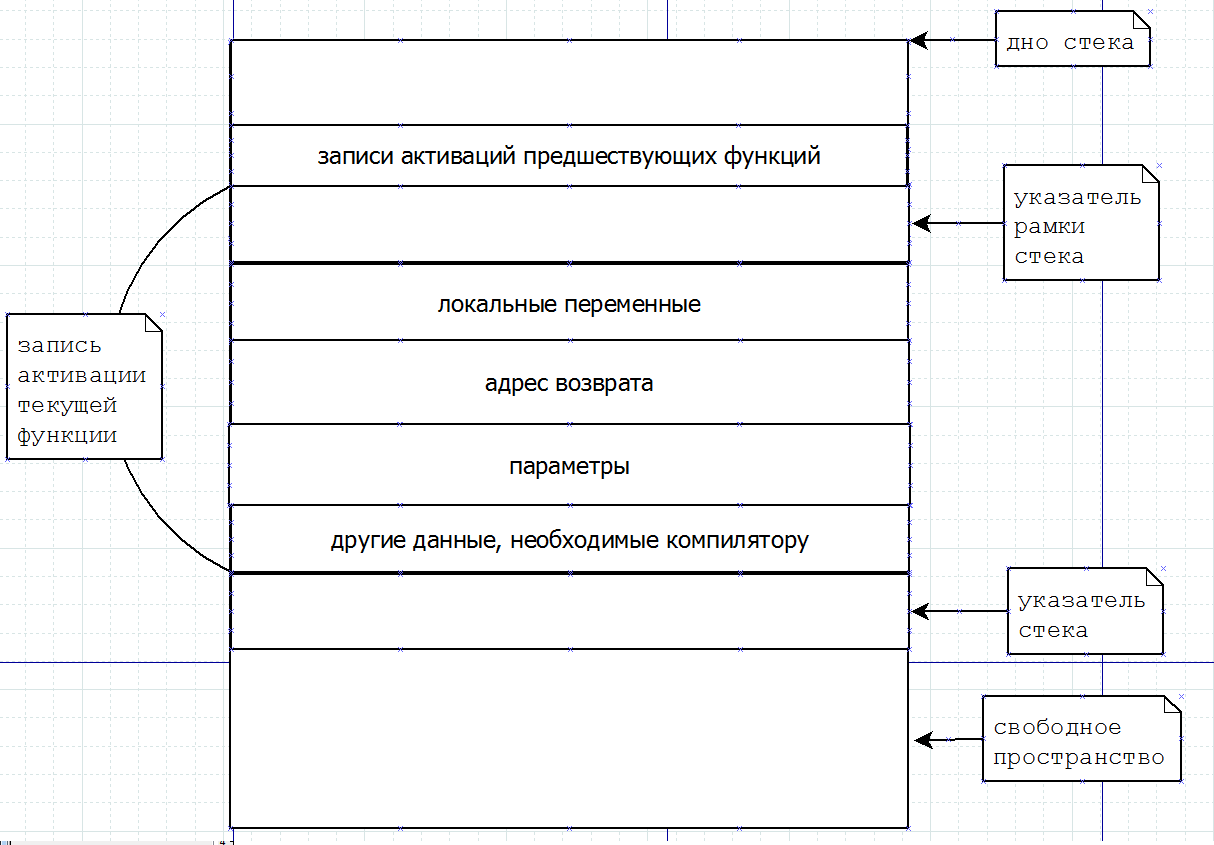
\includegraphics[width=0.8\textwidth]{Berezun/StackFrameC.png}
\caption{Стек языка C в реализации GCC.}
\end{figure}

Для построения точного корневого множества предлагается определить метаданные для каждой функции. Иными словами, предлагается хранить таблицу смещений 
локальных переменных и параметров относительно записи активации, которая будет вычисляться в самом начале работы программы и оставаться неизменной в 
течении всего времени её выполнения. При активации каждой функции на определенном смещении от указателя на её запись активации, заранее известном, в стек 
предлагается положить ссылку на эту таблицу или же просто хранить все эти таблицы в стеке, проассоциировав каждую из них с конкретной функцией. Таким образом 
для построения корневого множества необходимо будет просканировать стек, пройдясь по всем записям активации, и, пользуясь таблицей смещений для каждой функции, 
добавить все соответствующие элементы в корневое множество. При написании компилятора, точно зная разметку стека, данная идея реализуема, при использовании 
стороннего компилятора --- не всегда. Решение этой задачи могло бы быть следующим: явное указание программистом для каждой функции переменных, являющихся 
указателями; вычислив смещения этих переменных относительно записи активации функции, можно было бы занести их в её метаданные, и расположить их в записи 
активации в заранее известном месте. Однако GCC оптимизирует код, что не позволяет осуществить данную идею в чистом виде.

GCC производит оптимизацию кода на всех этапах компиляции. Точный набор оптимизаций меняется в каждой версии компилятора, но содержит стандартные алгоритмы 
оптимизации, такие как распределение регистров, планирование инструкций, оптимизация циклов и многие другие. При компиляции программы можно управлять оптимизацией 
с помощью специальных опций, однако компилятор будет оптимизировать распределение переменных в памяти в любом случае. Вне зависимости от порядка расположения в 
программном коде, компилятор будет располагать параметры и локальные переменные в записи активации подпрограммы в том порядке, который сочтёт оптимальным.
Порядок блоков в записи активации соблюдается всегда, т.е. сначала в стек кладутся локальные переменные, затем адрес возврата, параметры, другие данные, но 
внутри каждого из эти блоков порядок не определен.

Не существует явного порядка, согласно которому компилятор будет складывать локальные переменные в соответствующий блок. Более того, нет явного способа указать 
компилятору, чтобы последний положил необходимые нам метаданные на определенном смещении относительно записи активации. Но для функций, имеющих одинаковые параметры, 
тип и локальные переменные, при компиляции без оптимизации запись активации будет одинаковой, что позволяет вычислить метаданные в самом начале работы программы для 
каждой функции путем создания функции, имеющей такие же параметры и локальные переменные. Запустив такие функции в начале программы можно подсчитать все смещения и 
записать их в соответствующие таблицы смещений.

Ещё одной задачей является выявление записей активации в стеке. В GCC работа со стеком недоступна извне, поэтому выделить записи активации в програмном коде не 
представляется возможным. Несмотря на это, в режиме отладки можно использовать встроенные отладочные функции и различные функции трассировки. \emph{Трассировкой} 
называют список вызванных функций в активном потоке. В нашем случае предлагается ипользование следующих функций:

\begin{itemize}
\item \lstinline{void * __builtin_frame_address (unsigned int level)}. Возвращает адрес записи активации текущей функции или одной из функций, её вызвавших. 
Аргумент \lstinline{level} определяет номер записи активации в стеке, начиная с конца стека. Например:

\begin{itemize}
\item \lstinline{__builtin_frame_address (0)} вернёт адрес записи активации последней вызванной функции;
\item \lstinline{__builtin_frame_address (1)} --- функции её вызвавшей и т.д. 
\end{itemize}

Аргумент \lstinline{level} должен быть статической константой.

\item \lstinline{int *dladdr(void *addr, Dl_info *info)}. Записывает в \lstinline{info} имя и адрес фунции, имеющей адрес \lstinline{addr}. Значением данной 
фукнции является 1, если такая функция существует, 0 --- иначе.
\end{itemize}

При вызове функции построения корневого множества, функция \lstinline{__builtin_frame_address} позволяет обойти все записи активации, а функция \lstinline{dladdr} --- получить имена функций, им соответствующих. По имени функции ищется соответствующая ей метаинформация, используя таблицу смещений в которой строится корневое множество.

\section{Пример}

В данной секции описывается пример реализации вышеописанной идеи.

В следующем коде присутствуют две пользовательские функции \lstinline{f} и \lstinline{f2}. Функции
\lstinline{f_meta_calc} и \lstinline{f2_meta_calc} являются функциями вычисления метаинформации для функций
\lstinline{f} и \lstinline{f2} соотвественно; подобные функции должны быть описаны пользователем.

\begin{lstlisting}[mathescape=true]
#define _GNU_SOURCE
#define CALLSTACK_MAXLEN 64
#include <stdio.h>
#include <dlfcn.h>

// $\mbox{структура, возвращаемая для каждой функции в стеке}$
struct call {
    const void *address; // $\mbox{указатель рамки}$
	const char *function; // $\mbox{имя функции}$
};

// $\mbox{Структура, представляющая метаинформацию для некоторой функции.}$
typedef struct mm {
	int len; // $\mbox{количество указателей}$
// $\mbox{смещение указателей в записи активации относительно указателя}$
// $\mbox{на запись активации в стеке}$
	long *offsets;
} meta_table;
// $\mbox{метаинформация для каждой из функций}$
meta_table *f_meta_glob, *f2_meta_glob, *collect_meta_glob;

// $\mbox{регистр, в котором хранится текущий указатель рамки}$
// $\mbox{может меняться в зависимости от платформы}$
register void *rbp_reg asm ("rbp");
// $\mbox{функция вычисления смещения переменной x относительно указателя}$
// $\mbox{на текущую рамку}$
#define OFFS(x) (rbp_reg - (void*)&(x))

// $\mbox{структура, реализующая список;}$
// $\mbox{используется для хранения метаинформации функций}$
typedef struct tag_list List;
struct tag_list
{
	meta_table meta; // $\mbox{метаинформация}$
	char *function_name; // $\mbox{имя соответствующей функции}$
	List *next; // $\mbox{указатель на следующий элемент списка}$
	List *prev; // $\mbox{указатель на предыдущий элемент списка}$
};
// $\mbox{указатель на начало списка и конец списка}$
List *list_begin, *list_end;
// $\mbox{размер списка}$
int list_size;

// $\mbox{функция добавления элемента в список метаинформации}$
void add_element_to_the_end(meta_table mt, char *func_name) {
	List *new_element = (List*)malloc(sizeof(List));
	new_element->meta = mt;
	new_element->function_name = func_name;
	new_element->next = NULL;
	new_element->prev = list_end;
	
	if (!list_size)	{
		list_begin = new_element;
	} else {
		new_element->prev->next = new_element;
	}
	list_size++;
	list_end = new_element;
}

// $\mbox{функция трассировки}$
int backtrace(struct call trace[], int maxlen) {
	Dl_info dlinfo;
	unsigned int i;

	for (i = 0; i < maxlen; ++i) {
		switch (i) {
			case 0:
				if(!__builtin_frame_address(0)) {
					return i;
				}
				trace[i].address = __builtin_return_address(0);
				break;
			case 1:
				if(!__builtin_frame_address(1)) {
					return i;
				}
				trace[i].address = __builtin_return_address(1);
				break;
			case 2:
				if(!__builtin_frame_address(2))
					return i;
				trace[i].address = __builtin_return_address(2);
				break;
			case 3:
				if(!__builtin_frame_address(3))
					return i;
				trace[i].address = __builtin_return_address(3);
				break;
			case 4:
				if(!__builtin_frame_address(4))
					return i;
				trace[i].address = __builtin_return_address(4);
				break;
			case 5:
				if(!__builtin_frame_address(5))
					return i;
				trace[i].address = __builtin_return_address(5);
				break;
			case 6:
				if(!__builtin_frame_address(6))
					return i;
				trace[i].address = __builtin_return_address(6);
				break;
			case 7:
				if(!__builtin_frame_address(7))
					return i;
				trace[i].address = __builtin_return_address(7);
				break;
			case 8:
				if(!__builtin_frame_address(8))
					return i;
				trace[i].address = __builtin_return_address(8);
				break;
			/* etc */
			default:
				return i;
				break;
		}
		if (dladdr(trace[i].address, &dlinfo) != 0) {
			trace[i].function = dlinfo.dli_sname;
			trace[i].object = dlinfo.dli_fname;
		}
	}

	return i;
}

void* built_frame_address(unsigned int X) {
	switch (X){
		case 0:
			return __builtin_frame_address(0);
			break;
		case 1:
			return __builtin_frame_address(1);
			break;
		case 2:
			return __builtin_frame_address(2);
			break;
		case 3:
			return __builtin_frame_address(3);
			break;
		case 4:
			return __builtin_frame_address(4);
			break;
		case 5:
			return __builtin_frame_address(5);
			break;
		// ect //
	}
	return NULL;
}

// $\mbox{функция, возвращающая метаинформацию по имени функции;}$
// $\mbox{в случае, если функции с таким именем нет в списке, }$
// $\mbox{возвращается специальный объект meta\_table, }$
// $\mbox{у которого поле len равно -1}$
meta_table get_meta(char *func_name) {
	List *list_iterator = list_begin;
	meta_table mt;
	mt.len = -1;

	// $\mbox{обход списка метаинформаций}$
	while (list_iterator != NULL) {
		if (strcmp(list_iterator->function_name, func_name) == 0) {
			return list_iterator->meta;
		}
		list_iterator = list_iterator->next;
	}
	
	return mt;
}

// $\mbox{печать метаинформации по имени функции}$
void print_meta(char *name) {
	int i = 0;
	meta_table meta = get_meta(name);
	
	if (meta.len != -1) {
		for (i = 0; i < meta.len; i++) {
			printf(" offset[%i] = %li,", i, meta.offsets[i]);
		}
	} else {
		printf("No meta data defined for this function");
	}
	
}

// $\mbox{функция построения корневого множества}$
void collect() {
	printf("\ncollect starts\n");
	meta_table** meta = (meta_table**)alloca(sizeof(meta_table*));
	*meta = &collect_meta_glob;

	// $\mbox{выполняем трассировку}$
	struct call trace[CALLSTACK_MAXLEN];
	unsigned int i = 0;
	int depth = backtrace(trace, CALLSTACK_MAXLEN);
	
	printf("functions in stack:\n");
	// $\mbox{выводим информацию, полученную в результате трассировки}$
	for (i = 0; i < depth; ++i) {
		printf("%s: ", trace[i].function);
		printf(" fp = %p, ", built_frame_address(i + 1));
		print_meta(trace[i].function);
		printf("\n");
	}	
	
	printf("\ncollect end\n\n");
}

// $\mbox{функция вычисления метаинформации для функции f;}$
// $\mbox{последний параметр функции - вычисляемые метаданные}$
int f_meta_calc (int *a, int b, int *c, meta_table* meta) {
// $\mbox{инициализация всех переменных, которые заводятся в функции f;}$
// $\mbox{порядок следования аргументов и переменных у функции f и f\_meta\_calc}$
// $\mbox{должен быть одинаковый}$
	int z = 0;
	int z1 = 0;
	int z2 = 0;
	int *p;
	int *q; 

	// $\mbox{ручное заполнение метаинформации}$
	meta->len = 4;
	meta->offsets = (long*)malloc(sizeof(long) * meta->len);
	meta->offsets[0] = OFFS(a);
	meta->offsets[1] = OFFS(c);
	meta->offsets[2] = OFFS(p);
	meta->offsets[3] = OFFS(q);

	// $\mbox{печать построенной метаинформации}$
	printf("\nf_meta_calc starts:\n");
	printf ("  a %li \n", OFFS(a));
	printf ("  c %li \n", OFFS(c));
	printf ("  p %li \n", OFFS(p));
	printf ("  q %li \n\n", OFFS(q));
	printf("\nf_meta_calc end\n");
	return 0;
}

// $\mbox{вычисление метаинформации для функции f2;}$
// $\mbox{аналогична предыдущей функции}$
int f2_meta_calc (int *a, meta_table *meta) {
	int y = 0;
	int w = 0;
	int e = 2;

	meta->len = 1;
	meta->offsets = (long*)malloc(sizeof(long) * meta->len);
	meta->offsets[0] = OFFS(a);
	meta2 = (long)meta;

	printf ("\nf2 meta calc starts: \n");
	printf ("  a %li\n", OFFS(a));
	printf ("\nf2 meta calc end. \n");
	return 0;
}

// $\mbox{функция инициализации;}$
// $\mbox{вычисляет метаинформацию для всех функций}$
void init () {
	list_begin = list_end = NULL;
	list_size = 0;
	meta_table f_meta, f2_meta;
	
	// $\mbox{вычисление метаинформации функций f и f2}$
	f_meta_calc(0, 0, 0, &f_meta);
	f2_meta_calc (0, &f2_meta);
	
	// $\mbox{добавление метаинформации в список}$
	add_element_to_the_end(f_meta, "f");
	add_element_to_the_end(f2_meta, "f2");
} 
 
// $\mbox{пользовательская функция}$
int f (int *a, int b, int *c) {
	printf("\nf starts:\n");
	int z = 0;
	int z1 = 0;
	int z2 = 0;
	int *p;
	int *q;

	// $\mbox{некоторый код}$
     
	// $\mbox{вывод смещений указателей относительно указателя рамки;}$
	printf("rbp %p %p\n", rbp_reg, __builtin_frame_address(0));
	printf ("a %li \n", rbp_reg - (void*) &a);
	printf ("c %li \n", rbp_reg - (void*) &c);
	printf ("p %li \n", rbp_reg - (void*) &p);
	printf ("q %li \n", rbp_reg - (void*) &q);

	printf("\n f end \n");
	f2(a);
}

// $\mbox{пользовательская функция}$
int f2 (int*q) {
	int y = 0;
	int w = q[1];
	int e = 2;
	
	printf("\nf2 starts\n");
	printf("rbp %p %p\n", rbp_reg, __builtin_frame_address(0));
	printf ("q %li \n", OFFS(q));
	printf("\nf2 finish\n");

	collect();
}

int main (int argc, char **argv) {
	printf("main rbp %p\n", rbp_reg);
	int n;
	int * mas = (int*)malloc(sizeof(int) * 4);

	init ();

	f(mas, mas, mas);
  
	return 0;
}
\end{lstlisting}

В результате с помощью метаинформации, описанной пользователем, функция \lstinline{collect} выведет указатели
рамки и смещения указателей функций относительно этой рамки. Можно видеть, что эти данные совпадают с данными,
выводимыми во время работы самих функций. Т.о. функция \lstinline{collect} выводит текущее точное корневое
множество.

\section*{Заключение}

Построение корневого множества является плаформозависимой операцией. В простейшем случае необходимо просканировать 
регистры, стек и статические данные, добавив все указатели в кучу в корневое множество. В данной работе была описана 
организация стека и рассмотрены процессы построения корневого множества в языке OCaml и консервативном сбощике мусора 
для C/C++ BoehmGC. Было предложено решение задачи построения точного корневого множества для языка C с помощью метаинформации, 
строящейся при помощи пользователя, и приведен пример такого построения с использованием компилятора GCC.

\begin{thebibliography}{99}
\bibitem{ref1}  
Naveen Sharma, Sanjiv Kumar Gupta. 
Optimal Stack Slot Assignment in GCC. GCC Summit, 2003.

\bibitem{ref2}
Fridtjof Siebert. 
Realtime Garbage Collection in the JamaicaVM 3.0. 5th International Workshop on Java Technologies for Real-Time and Embedded Systems, 2007.

\bibitem{ref3}
Terrence W.Pratt, Marvin V.Zelkowitz. 
Programming Languages Design and Implementation. Prentice Hall PTR, 2004.

\bibitem{ref4}  
William Pugh. Skip Lists: a Probabilistic Alternative to Balanced Binary Trees. Communications of the ACM, Vol. 33 No. 6, 1990.
\end{thebibliography}
